\section{Brief reflection}
\textit{"A brief reflection on your progress so far, and an overview of the remaining work. Which circuits do you have to design/implement? Which simulations are you planning to run? Are there any parts of the work that you have already done that you plan to improve/change?"}

We have focused extensively on Verilog, and thus implemented the 8x8 memory completely and done testing on its functionality. We started out with a different design and have iterated on it several times. The architecture is close, but somewhat different, to the specifications requested, since the task says "should" and not "shall". Here is a testbench for the entire 8x8 memory:

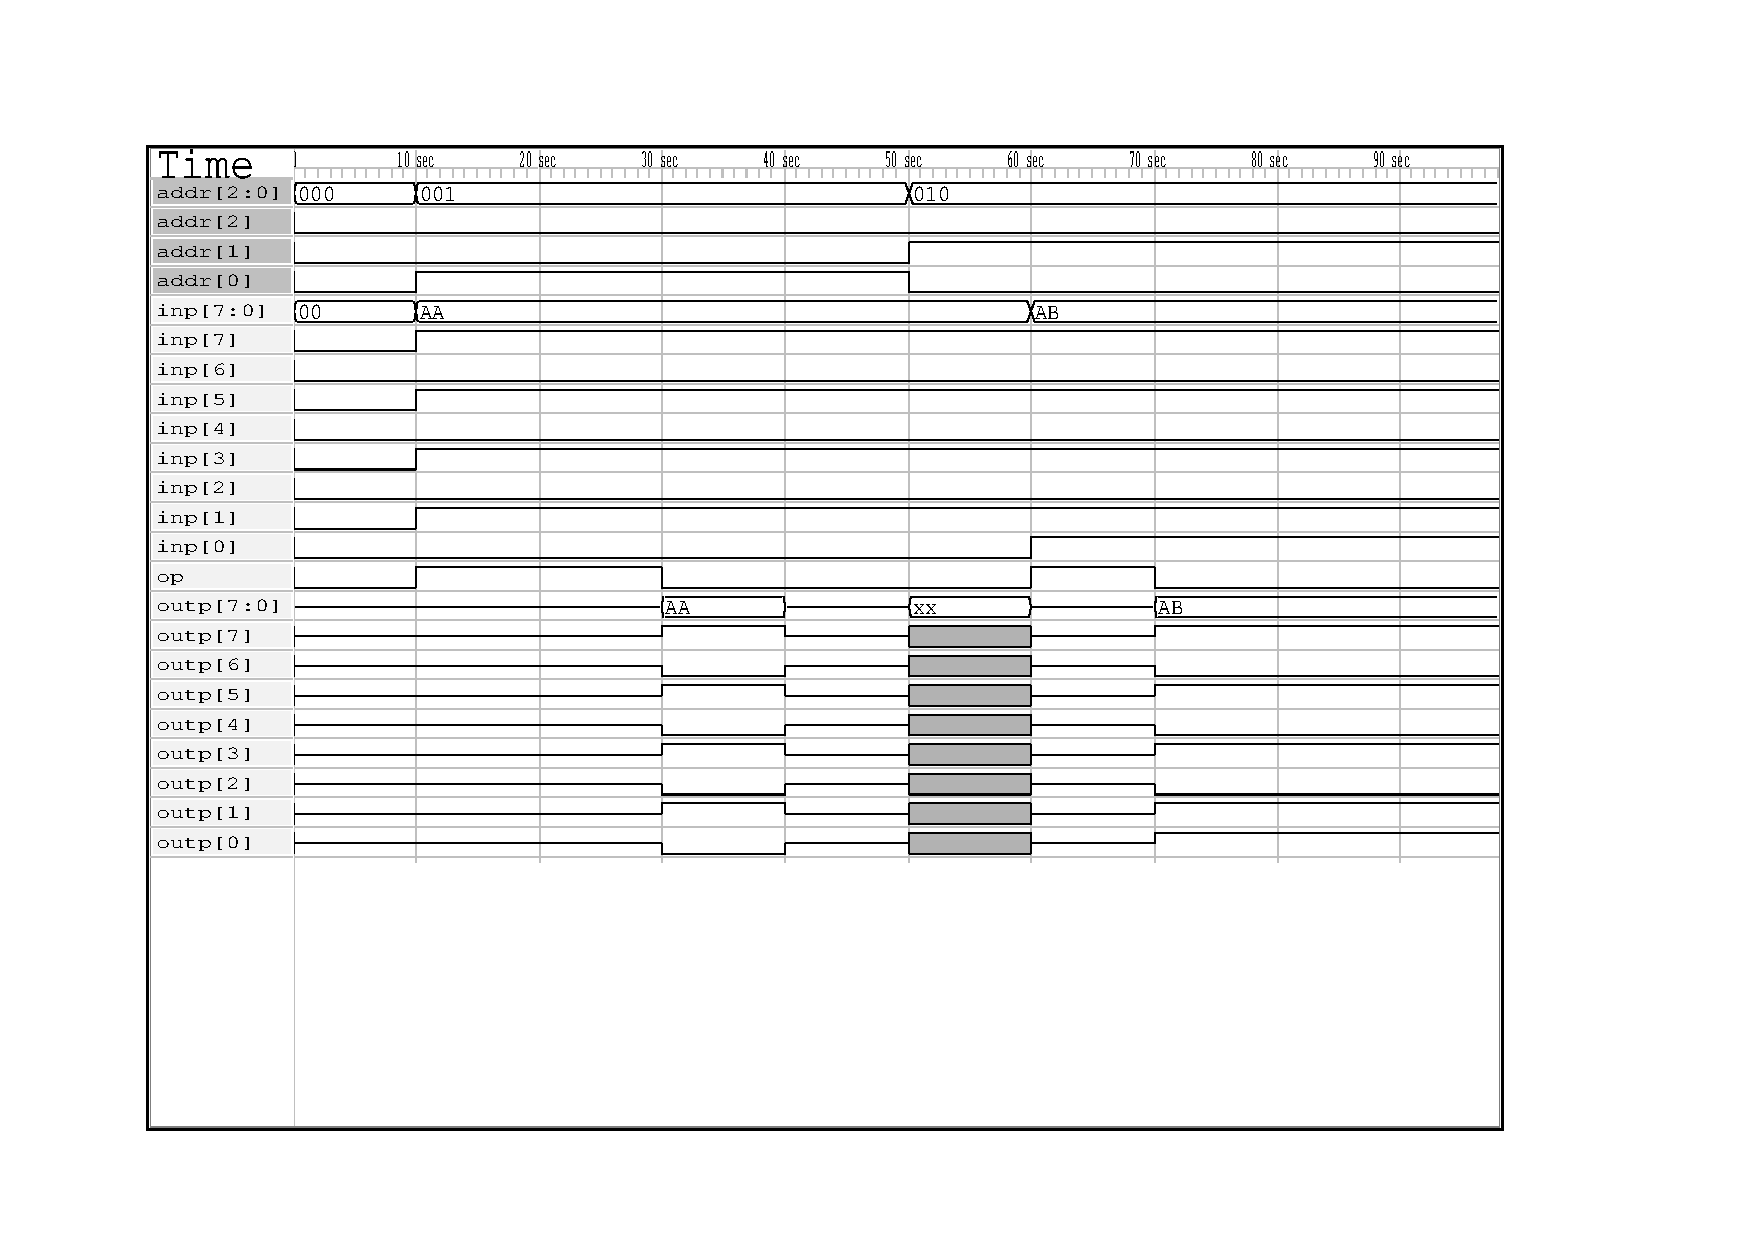
\includegraphics[width=\textwidth]{verilog_mem8x8_latch/simple_testbenches/ram.pdf}

We have however yet to implement the FSM. And after that is implemented we will set up a testbench that completes all of the digital circuitry testing, such as writing our own initials in ASCII into the memory.

When it comes to AimSPICE we are somewhat stuck, as both of us have done the bare minimum of AimSPICE-ing to pass the exercises thus far, and will do more AimSPICE after consulting the TAs. What an ancient language and editor that language has. Our frustration with PainSPICE is immesureable, and my week is ruined. Had there just been somewhat of a linter available. Ignore our rants for now, and make sure to send as many TAs to øvingstime as possible, and we will tame the beast known as AimSPICE before the project deadline.

We have however taken analog design principles into account in our digital design, so the analog simulations should perform well. We are a bit worried about how fast the bitcell flips values, but that is all.
